% pilot
The Rhode Island Board of Elections performed a pilot audit in Providence 
in February 2022. The contest audited was a single yes-or-no question in the November 2021 election: Portsmouth's
Issue 1, "School Construction and Renovation Projects". The question had a reported margin of $0.2567$ and the audit used a risk-limit of $0.10$.

A first round size of $140$ ballots with large probability of stopping ($0.95$) was selected.
Selection order was tracked for the sake of analysis.
As expected, the audit concluded in the first round. The \Providence risk was $0.0418$. Table~\ref{tab:pilot-risks} shows risk measures for the drawn sample using \Providence, \Minerva and \BRAVO (both EoR and SO).

\begin{table}[h!]
\begin{center}
\begin{tabular}{ |c|c|c|c|c| } 
\hline
%\diagbox[dir=NW]{First \\Round \\Size}{RLA}
ballots& \rotatebox{45}{\Providence} & \rotatebox{45}{\Minerva} & \rotatebox{45}{SO \BRAVO} & \rotatebox{45}{EoR \BRAVO} \\
\hline
140 & \bf{0.0418} & \bf{0.0418} & \bf{0.0541} & 0.366 \\
\hline
\end{tabular}
\end{center}
\caption{Risk measures for the drawn first round of $140$ ballots in the Providence, RI pilot audit. Risks in bold meet the risk-limit ($10\%$) and thus correspond to audits that would stop.}
\label{tab:pilot-risks}
\end{table}

Note that the risk measures shown in Table~\ref{tab:pilot-risks} imply that, for the sample obtained in the pilot audit, an EoR \BRAVO audit would not have stopped in the first round, despite the large round size. Further, if the risk limit had been $0.05$ instead of $0.10$, SO \BRAVO also would have required moving on to a second round. 

We can use simulations to better understand typical audit behavior for the margin of this pilot audit and contextualize the results we obtained in the pilot. We run $10^4$ trial audits for several stopping probabilities $p$. Each round size is chosen to give a probability of stopping $p$ assuming the announced tally and given the results of previous rounds. We use the same $0.1$ risk limit and margin of $0.2557$. 

Figure~\ref{fig:pilot_sims} shows the average number of ballots sampled for each value of $p$ in the simulations. The vertical line denotes the stopping probability of the first round size actually chosen in the pilot ($140$ ballots). The large value of $p$ corresponds to a large first round size and a corresponding large value of average number of ballots. In later sections we show why average number of ballots is not the only metric to optimize, and how large round sizes can be beneficial from the perspective of other important metrics. 
%The average number of ballots for such a high stopping probability round schedule is high. For the first round size used in the pilot there was an approximately $0.95$ probability of stopping, and consequently, in Figure~\ref{fig:pilot_sims}, this corresponds to a higher average total ballots sampled than lower values of $p$. Of course, average number of ballots is not the only metric that matters when planning an audit. 

\begin{figure}
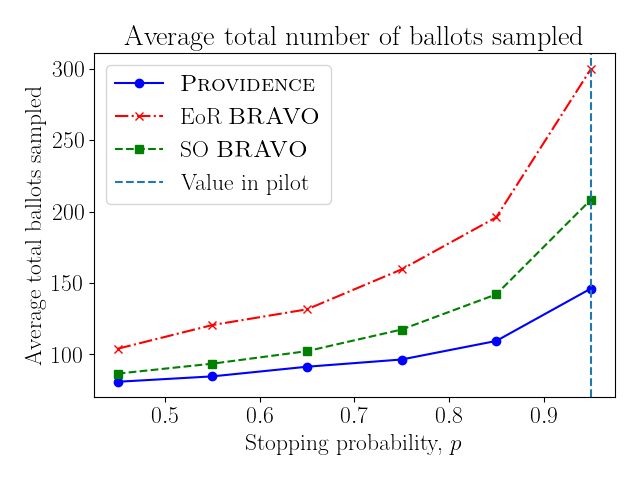
\includegraphics[width=.5\textwidth]{pilot_sims.png}
\caption{The total number of ballots sampled on average in our audit simulations using the same contest parameters and risk limit as the Rhode Island pilot. The average total ballots are shown for various round schedules, parameterized by $p$, the conditional stopping probability used to select each round size.}
\label{fig:pilot_sims}
\end{figure}


For this pilot audit, extensive planning of the round schedule was not necessary because the margin was large enough that relatively few ballots were needed to achieve the high probability of stopping. In Section~\ref{sec:workload} we consider a larger state-wide contest in Virginia, where selecting the round schedule has more significant implications. Virginia also currently uses ballot polling RLAs, whereas Rhode Island primarily uses batch comparison RLAs. Some of the ideas introduced in Section~\ref{sec:workload} provide a context for this pilot case as well.

For the sake of analysis, the selection order of the ballots sampled during the pilot was also recorded. Figure~\ref{fig:pilot_sequence} shows the cumulative tally of winner ballots after each new ballot in the selection order is added to the sample. We observe two interesting phenomena in this particular sample's selection order. 
\begin{description}
\item First, an SO \BRAVO audit of this sample stops because the \BRAVO condition is met when the sample (orange line) surpasses the minimum number of winner ballots (blue line) earlier in the sample.\footnote{Such cases also provide insight into how \Providence is a tighter test in expectation because SO \BRAVO ignores information from the rest of the sample after the \BRAVO condition is met at some point earlier in the selection order.} EoR \BRAVO, however, does not stop. It might be difficult to explain to the public why SO \BRAVO stops in more extreme cases like this, where the condition is met early in the sample, but poor evidence for the alternative hypothesis in the rest of the sample is ignored. 
\item Second, only $5$ of the first $11$ ballots were for the announced winner. A first round of size $11$ would have provided misleading evidence due to a too-small sample size. 
\end{description}
Both these ideas are addressed more thoroughly in Section~\ref{sec:workload}.
%first draft, needed to be shorter: ...stopping condition for the cumulative tally at the end of the round would see that the \BRAVO condition is not met (and would be correct that an EoR \BRAVO audit would require a second round for this sample). On the other hand, an SO \BRAVO audit does stop already in the first round because the cumulative sample met the \BRAVO stopping condition at some point before all the ballots had been added to the sample. In Figure~\ref{fig:pilot_sequence}, this is seen when the observed sample (orange) line touches (or goes above) the minimum winner ballots (blue) line which gives the \BRAVO stopping condition (i.e. a \BRAVO condition is met whenever the number of winner ballots in the sample is at least the number indicated by that blue line). While relatively rare, there also possible cases of selection order where the SO \BRAVO condition is met very early but then bad luck is had thereafter and the ultimate cumulative sample at the end of the round gives very poor evidence that the announced tally is correct. There could even be fewer ballots for the winner than the loser. Such cases might be difficult for an election official to explain to the public, especially when the evidence at the end of the round provides poor support for the alternative hypothesis.\footnote{Such cases also provide insight into how \Providence is a tighter test in expectation because SO \BRAVO ignores information from the rest of the sample after the \BRAVO condition is met at some point earlier in the selection order.} In Section~\ref{sec:workload} we address such cases more thoroughly.

\begin{figure}
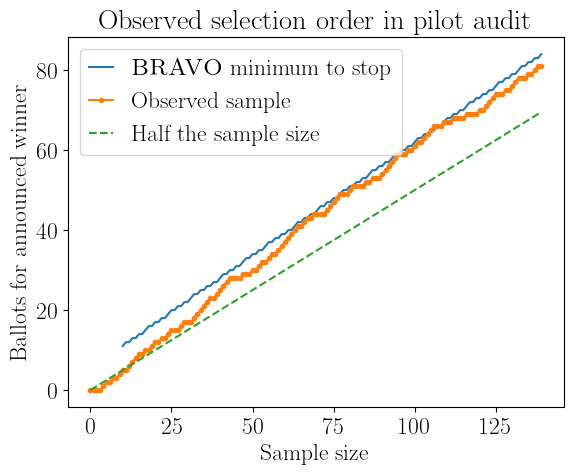
\includegraphics[width=.5\textwidth]{pilot_sequence.png}
\caption{For each sample size from $1$ to $140$, the intermediate cumulative sum of ballots for the announced winner found in the sample is shown.}
\label{fig:pilot_sequence}
\end{figure}




